
\section{Modelo Identificado}


\begin{frame}{Observação}
\begin{itemize}
\item 2 horas 
\item 4.5 ciclos ~120 cubos
\item 65 Entradas e Saídas
\item 19751 vetores registrados
\item 1321 vetores únicos
% cat 2019-05-10_1524NoTimeIOheader.csv | cut -d, -f1 --complement | sort -V | uniq | wc -l
\end{itemize}\end{frame}


\begin{frame}{Modelo Identificado}
\begin{itemize}
\item 2 caminhos 
\end{itemize}
\begin{figure}[H]
  \centering
  \includegraphics[width=0.5\textwidth]{results/all/states.pdf}
  \caption{Variação de número de estados em relação ao valor de $k$.}
    \label{fig:statesIdentOriginal}
\end{figure}
\end{frame}

\begin{frame}{Modelo Identificado}
\begin{figure}[H]
  \centering
  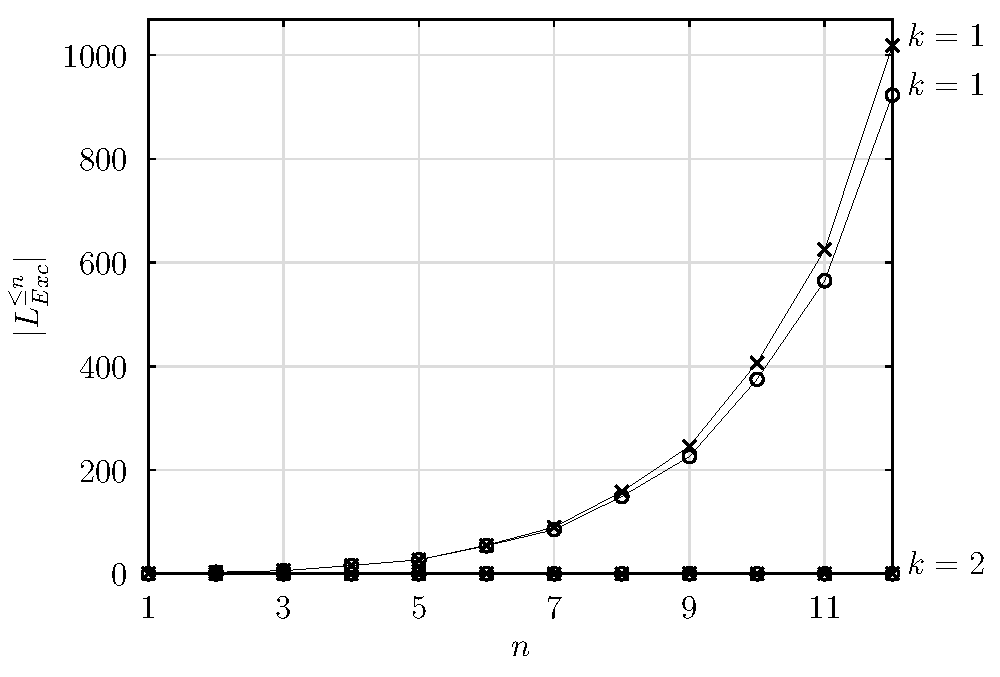
\includegraphics[width=0.5\textwidth]{results/all/exceedingLanguage-daoct-ndaao_k1-2_n12.pdf}
  \caption{Linguagens Excedentes - DAOCT (o), NDAAO ($\times$).}
    \label{fig:daoctNdaaoOriginal}
\end{figure}
\end{frame}


\begin{frame}
\begin{itemize}
\item Verificar comportamento ao trocar vetor inicial \pause
\item Escolhido o vetor com maior incidência
\end{itemize}
\end{frame}

\begin{frame}{Observação - Arquivo modificado}
\begin{itemize}
\item 19427 vetores registrados
\item 1294 vetores únicos
% cat 2019-05-10_1524NoTimeIOheader.csv | cut -d, -f1 --complement | sort -V | uniq | wc -l
\end{itemize}
\end{frame}

\begin{frame}{Modelo Identificado - Arquivo Modificado}
\begin{itemize}
\item 80 caminhos 
\end{itemize}
\begin{figure}[H]
  \centering
  \includegraphics[width=0.5\textwidth]{results/all/best/states.pdf}
  \caption{Variação de número de estados em relação ao valor de $k$.}
    \label{fig:statesIdentOriginal}
\end{figure}
\end{frame}

\begin{frame}{Modelo Identificado - Arquivo Modificado}
   \begin{figure}[ht]
       \begin{minipage}[b]{0.35\linewidth}
         \centering
    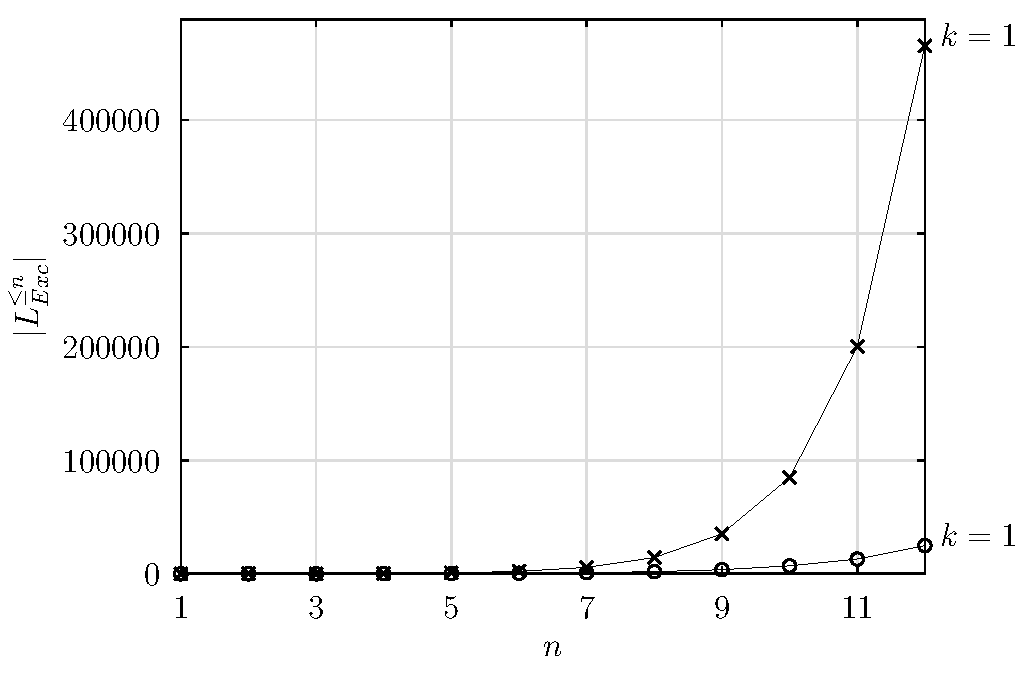
\includegraphics[width=\textwidth]{results/all/best/exceedingLanguage-daoct-ndaao_k1_n12.pdf}
\end{minipage}
       \begin{minipage}[b]{0.35\linewidth}
         \centering
    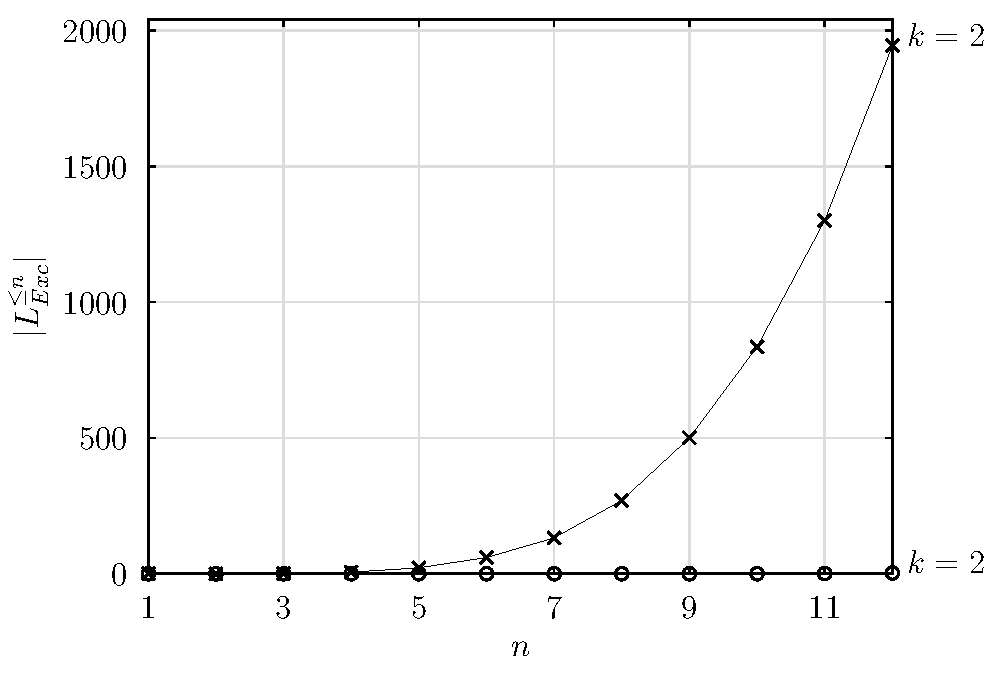
\includegraphics[width=\textwidth]{results/all/best/exceedingLanguage-daoct-ndaao_k2_n12.pdf}
       \end{minipage}
       \hspace{0.5cm}
       \begin{minipage}[b]{0.35\linewidth}
           \centering
    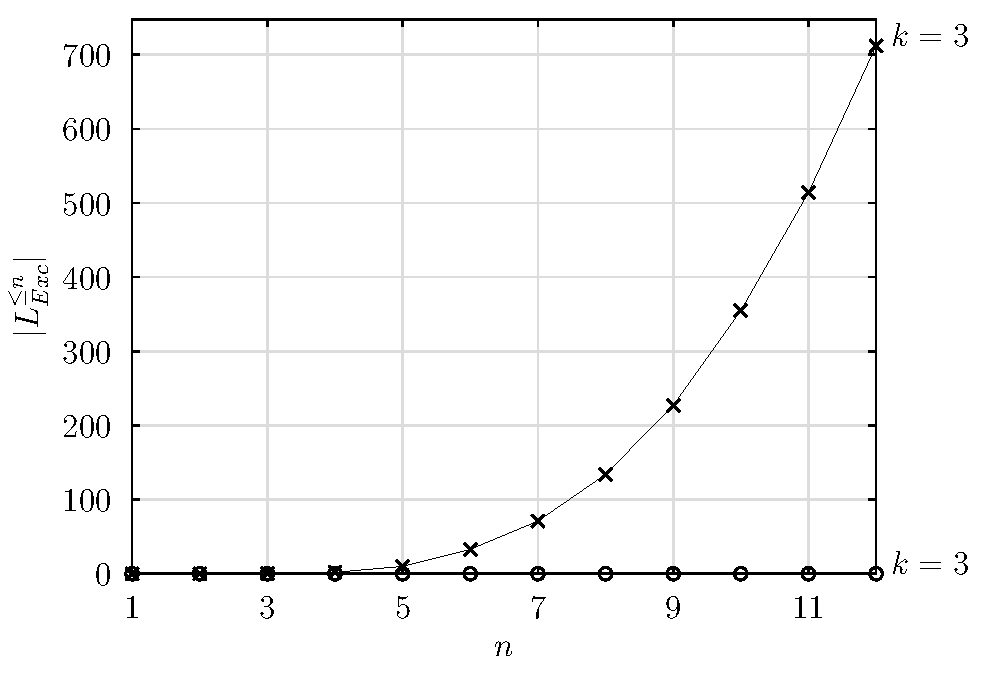
\includegraphics[width=\textwidth]{results/all/best/exceedingLanguage-daoct-ndaao_k3_n12.pdf}
       \end{minipage}
       \begin{minipage}[b]{0.35\linewidth}
           \centering
    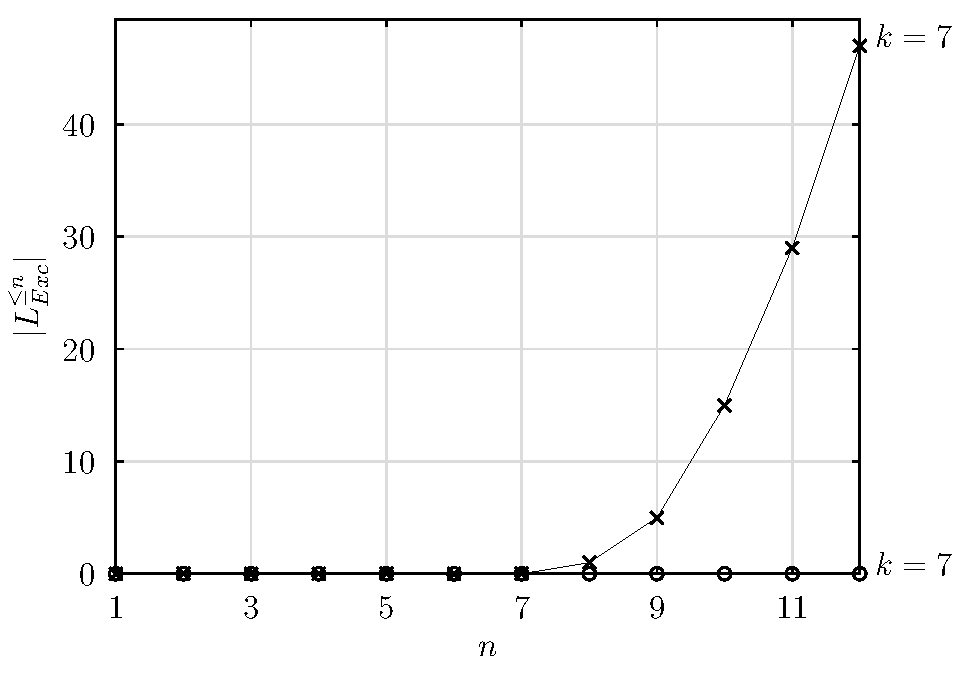
\includegraphics[width=\textwidth]{results/all/best/exceedingLanguage-daoct-ndaao_k7_n12.pdf}
       \end{minipage}
  \caption{Linguagens Excedentes - DAOCT (o), NDAAO ($\times$).}
   \end{figure}
\end{frame}


\begin{frame}{Discussão Escolha Vetor inicial}
\begin{figure}[H]
  \centering
  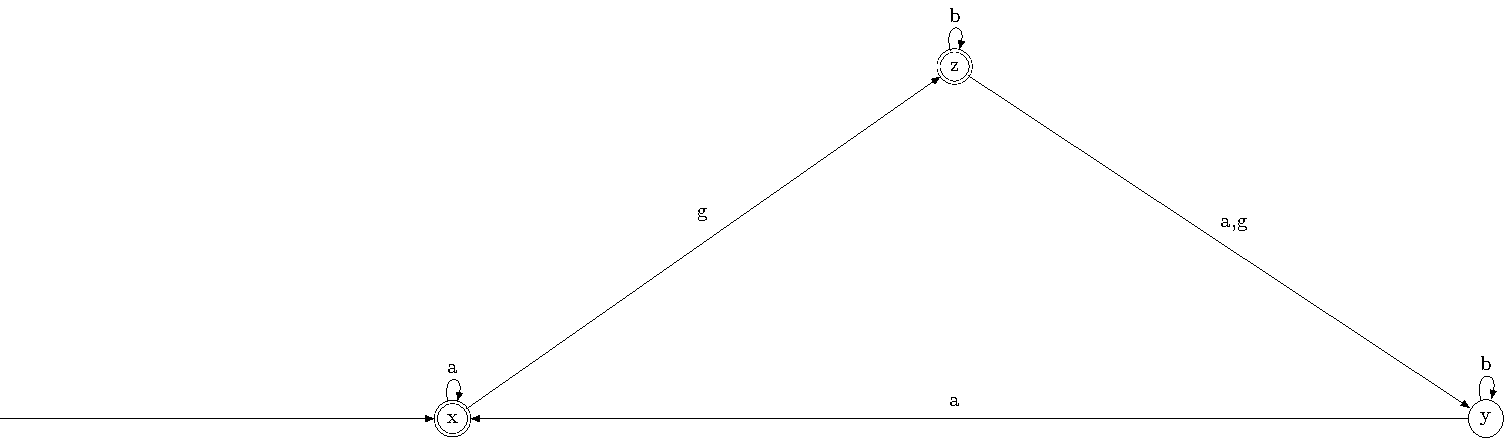
\includegraphics[width=.5\textwidth]{results/example/example}
  \caption{Scheme of the example.}
    \label{fig:schemeExConveyor}
\end{figure}
\end{frame}

\begin{frame}{Discussão Escolha Vetor inicial}
\begin{align*}
  \label{motif}
{\only<2>{\color{gray}} {\only<4>{\color{blue}}\colvec{0\\0\\0}}\colvec{1\\0\\0}\colvec{0\\0\\0}\colvec{0\\1\\0}\colvec{0\\0\\0}\colvec{0\\0\\1} }
\only<1,2>{\colvec{0\\0\\0}\colvec{1\\0\\0}\colvec{0\\0\\0}\colvec{0\\1\\0}\colvec{0\\0\\0}\colvec{0\\0\\1}}
\end{align*}
\end{frame}


\begin{frame}{Discussão Escolha Vetor inicial}
\begin{figure}[H]
  \centering
 \includegraphics[height=0.5\textheight]{results/example/examplek1NoArrows}
  \caption{Identified model using $\colvec{0&0&0}^T$ as initial state, $k=1$.}
    \label{fig:exampleCol000k1}
\end{figure}
\end{frame}

\begin{frame}{Discussão Escolha Vetor inicial}
\begin{align*}
{\only<2>{\color{blue}}\colvec{1\\0\\0}}\colvec{0\\0\\0}\colvec{0\\1\\0}\colvec{0\\0\\0}\colvec{0\\0\\1}\colvec{0\\0\\0}
\end{align*}
\end{frame}

\begin{frame}{Discussão Escolha Vetor inicial}
\begin{figure}[H]
  \centering
  \includegraphics{results/example/example1k1NoArrows}
  \caption{Identified model using $\colvec{1&0&0}^T$ as initial state, $k=1$.}
    \label{fig:exampleCol100k1}
\end{figure}
\end{frame}


% \begin{frame}{Discussão Escolha Vetor inicial}
% \begin{figure}[H]
%   \centering
%   \includegraphics[width=\textwidth]{results/example/example1k2NoArrows}
%   \caption{Identified model using $\colvec{1&0&0}^T$ as initial state, $k=2$.}
%     \label{fig:exampleCol100k2}
%   \end{figure}
% \end{frame}



%%% Local Variables:
%%% mode: latex
%%% TeX-master: "../presentation"
%%% End: